\documentclass[10pt]{article}
\usepackage{float}
\RequirePackage{eso-pic}
\usepackage{caption}
\captionsetup[table]{labelformat=empty}



\usepackage{geometry}
\geometry{
a4paper,
left=11mm,
right=14mm,
top=37mm,
bottom=14mm,
}



\usepackage{colortbl}
\usepackage{fontspec}
\setmainfont[Ligatures=TeX]{Calibri}



\newcommand\BackgroundPic{%
\put(0,0){%
\parbox[b][\paperheight]{\paperwidth}{%
\vfill
\centering
\includegraphics{MBIE_generic_background.pdf}%
\vfill
}}}



\begin{document}
\thispagestyle{empty}
\AddToShipoutPicture{\BackgroundPic}
\section*{Key Export Statistics\footnotemark - Cane Beet Sugar\footnotemark }
Published on April 11, 2016. \par
\small{\noindent{\textit{Monthly data from January 2000 to November 2015.}}}
\begin{table}[ht]
\centering
{\scriptsize
\begin{tabular}[t]{p{1.8cm}>{\hfill}p{1.4cm}>{\hfill}p{1.4cm}>{\hfill}p{1.6cm}>{\hfill}p{1.9cm}>{\hfill}p{2cm}>{\hfill}p{1.9cm}>{\hfill}p{1.5cm}}
 \textbf{Country} & \textbf{Yearly Qty} & \textbf{Yearly Value} & \textbf{Yearly Price} & \textbf{3Year CAGR(Qty)} & \textbf{3Year CAGR(Value)} & \textbf{3Year CAGR(Price)} & \textbf{Price Elasticity} \\
\hline
French Polynesia & 6,059 & 5.2 & \$0.9 & 1.2\% & -24\% & -25\% & 0.0 \\  
Solomon Islands & 4,560 & 4.3 & \$0.9 & 9.4\% & -3.4\% & -11.7\% & -0.8 \\  
New Caledonia & 3,308 & 3.1 & \$0.9 & -17.8\% & -25.2\% & -8.9\% & 2.0 \\  
Fiji & 2,453 & 2.1 & \$0.8 & 70.1\% & 47\% & -13.6\% & -5.2 \\  
Samoa, American & 981 & 1.0 & \$1.1 & -6.1\% & -13.1\% & -7.4\% & 0.8 \\  
Malaysia & 666 & 0.5 & \$0.7 & -49.7\% & -55.5\% & -11.6\% & 4.3 \\  
Other & 1,873 & 2.0 & \$1.1 & -56.1\% & -60.2\% & -9.2\% & 6.1 \\  
Total & 19,901 & 18.2 & \$0.9 & 50.5\% & 15.1\% & -23.5\% & -2.1 \\  
\hline
\end{tabular}
}
\caption{\scriptsize Top 6 Cane Beet Sugar Markets for year ending November - 2015: Quantity('000 kg) Value(NZ\$Mill), Price and their last 3-Year Growth Rates}
\end{table}


\vspace{-0.7cm}



   \begin{figure}[H]
   \centering
    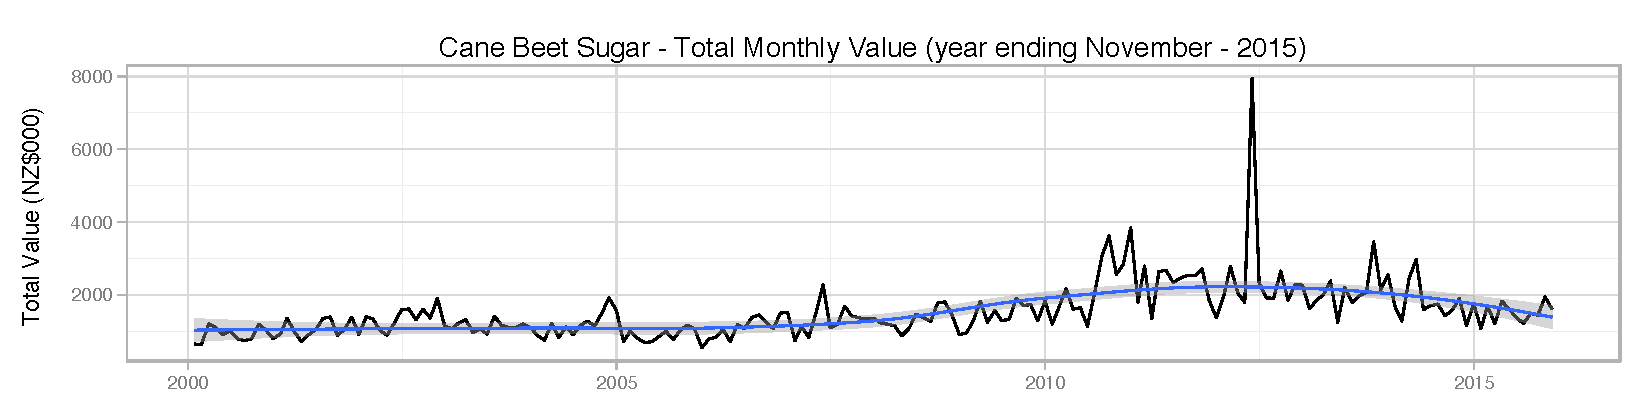
\includegraphics[scale=0.53]{../graphs/monthly_value/cane_beet_sugar_monthly_value.pdf} \
    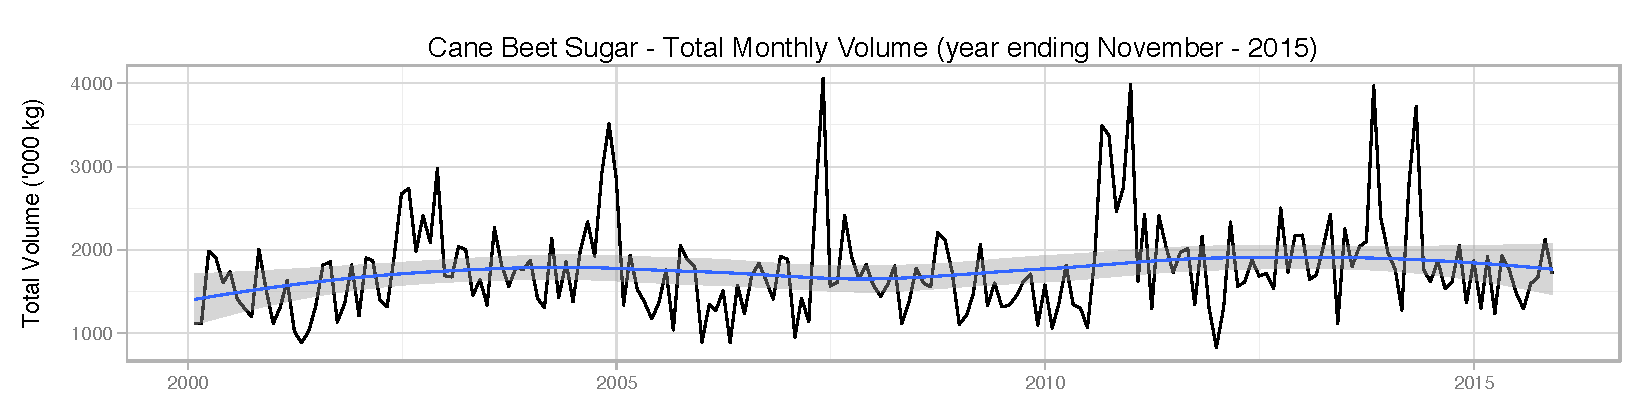
\includegraphics[scale=0.53]{../graphs/monthly_volume/cane_beet_sugar_monthly_volume.pdf} \
    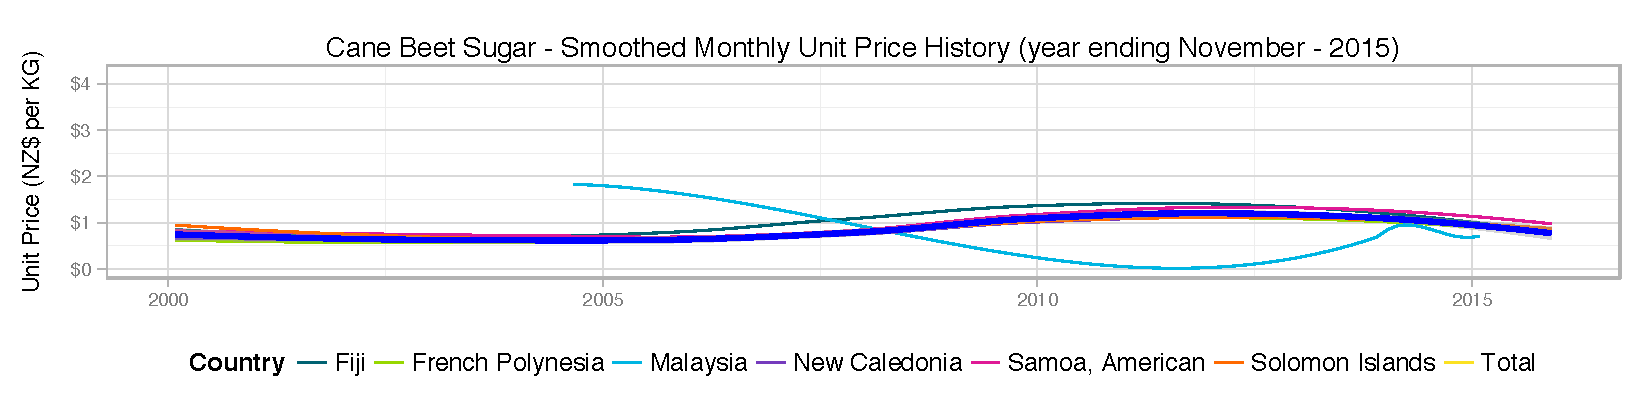
\includegraphics[scale=0.53]{../graphs/smoothed_price/cane_beet_sugar_smoothed_price.pdf} \
    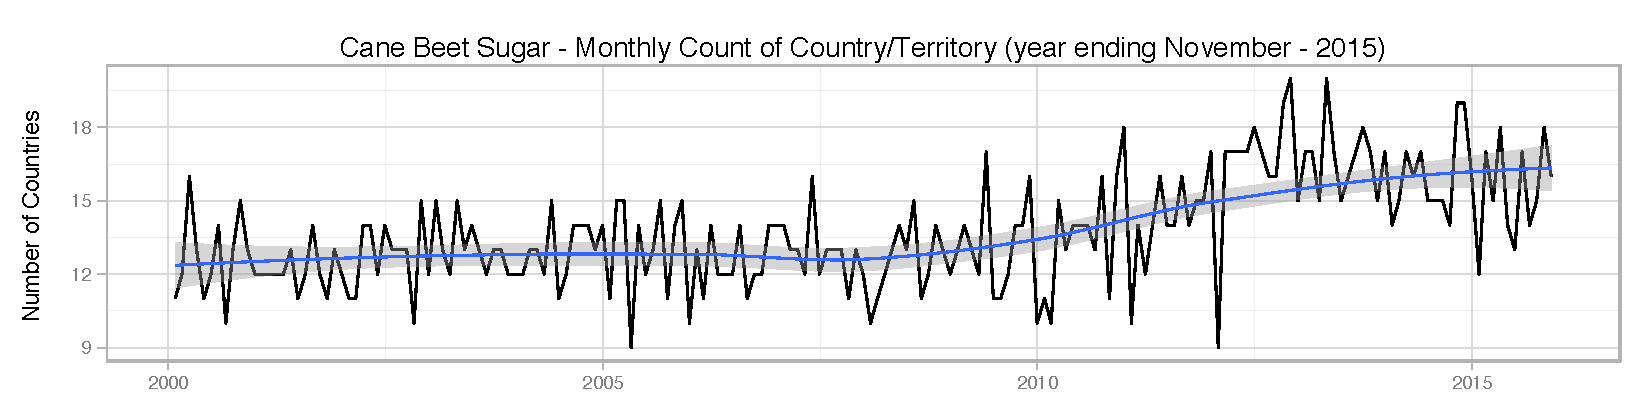
\includegraphics[scale=0.53]{../graphs/monthly_number_countries/cane_beet_sugar_monthly_count.pdf} \
    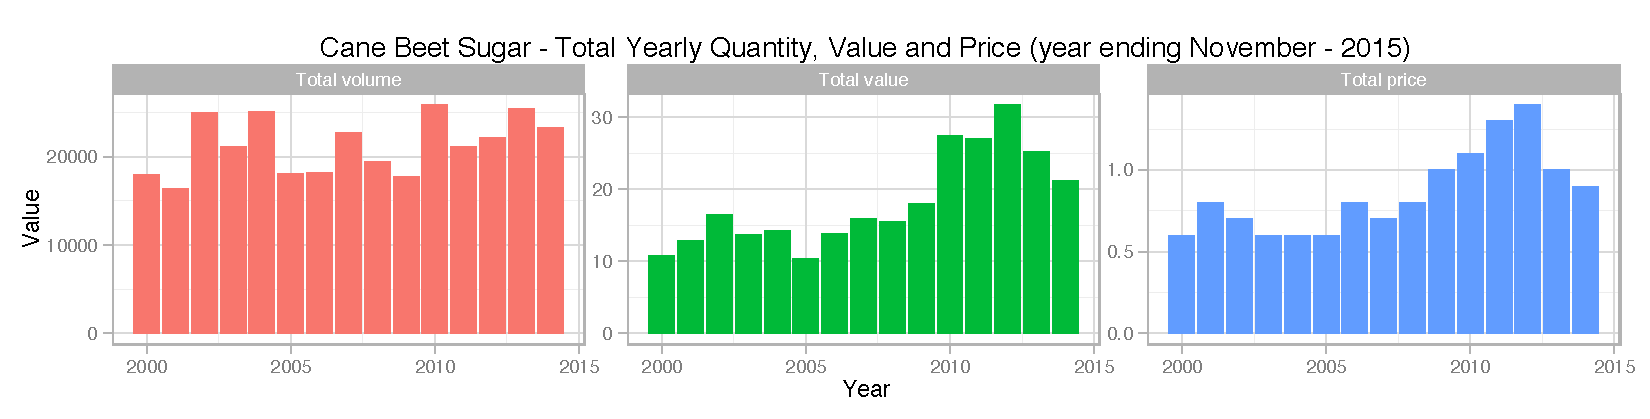
\includegraphics[scale=0.53]{../graphs/yearly_summary/cane_beet_sugar_yearly_summary.pdf} \
   \end{figure}



\footnotetext[1]{Source: Statistics New Zealand - Overseas Merchandise Trade}
\footnotetext[2]{Harmonised System Codes for Cane Beet Sugar starting with: 170199.}
\end{document}
